%=======================================================================
\section{\code{Physics} class}
%=======================================================================


\subsection{Attributes}

\subsection{Operations}

%=======================================================================
\section{\code{Domain} class}
%=======================================================================


\subsection{Attributes}

\subsection{Operations}

%=======================================================================
\section{\code{BC} class}
%=======================================================================

The \code{BC} class defines boundary conditions on a \code{Domain}.



\subsection{Attributes}

\subsection{Operations}

%=======================================================================
\section{\code{IC} class}
%=======================================================================

The \code{IC} class defines initial conditions for a set of
\code{Field}s in a \code{Domain}.


\subsection{Attributes}

\subsection{Operations}

%=======================================================================
\section{\code{Problem} class}
%=======================================================================

The \code{Problem} class defines the problem to be solved, including
the domain, boundary conditions, and initial field values.


\subsection{Attributes}

\subsection{Operations}

%=======================================================================
\section{\code{Field} class} \label{ss:field}
%=======================================================================

A \code{Field} represents a discrete multiresolution scalar or vector
field.  A \code{Field} is associated with a \code{Hierarchy}, and is
composed of \code{Array}'s defined on a subset of \code{Grid}s in the
\code{Hierarchy}.

\subsection{Attributes}

\subsection{Operations}

%=======================================================================
\section{\code{Units} class}
%=======================================================================

A \code{Units} class represents the physical units for the data in a
\code{Field}.

\subsection{Attributes}

\subsection{Operations}

\newpage

%======================================================================@
\chapter{Data Classes} \label{s:data-classes}
%======================================================================@

\centerline{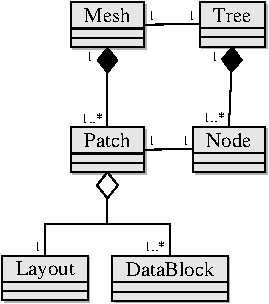
\includegraphics{uml/amr.1}}

%=======================================================================
\section{\code{Hierarchy} class}
%=======================================================================

A \code{Hierarchy} class represents a distributed structured AMR grid
hierarchy.  A \code{Hierarchy} can be considered to be an aggregate of
\code{Level}s, each of which in turn is an aggregate of individual
\code{Patch}es.  A patch is composed of a \code{Box}, which defines
the position and size in space, and some number of \code{Array}s, which
are used to store \code{Field} data (see \S\ref{ss:field}).



\subsection{Attributes}

\subsection{Operations}

%=======================================================================
\section{\code{Level} class}
%=======================================================================

A \code{Level} class represents a level in a distributed structured
AMR grid hierarchy (\code{Hierarchy}, where a level is defined as all
grid patches (\code{Grid}s) that have the same resolution.  A
\code{Level} is usually contained in a \code{Hierarchy}.

% The AMR hierarchy is represented using the trio of classes
% \code{Hierarchy}, \code{Level}, and \code{Grid}.
%   A \code{Grid} is a
% box in space, and is decomposed into \code{GridLocal} and
% \code{GridRemote} classes (see \S\ref{sss:class-grid}).  Each
% \code{GridLocal} object has some number of \code{Field} objects
% associated with them (see \S\ref{sss:class-field}), though the
% \code{GridLocal} objects themselves do not store field data
% themselves.  A \code{Level} class is also either a ``structured''
% \code{LevelStruct} or an ``unstructured'' \code{LevelUnstruct}.
% Structured levels are composed of a regular array of \code{Grid}s, and
% is typically used for unigrid calculations or the root level of an AMR
% calculation.  Unstructured levels are typically used for non-root
% levels of an AMR calulation.

\subsection{Attributes}

\subsection{Operations}

%=======================================================================
\section{\code{Patch} class}
%=======================================================================

A \code{Patch} class represents a grid patch in a distributed structured
AMR grid hierarchy (\code{Hierarchy}).  A \code{Patch} is defined by a
\code{Box}, and a set of \code{Array}s defined on the \code{Patch}.  Each
\code{Patch} is contained within a \code{Level}, and may be distributed
according to a \code{Parallel} object.

\subsection{Attributes}

\subsection{Operations}

%=======================================================================
\section{\code{Box} class}
%=======================================================================

The \code{Box} class is for representing a box, and provides KeLP-like functionality.
Boxes are determined by two points, which may be of any parameterized type
(e.g.~\code{int} or \code{double}, etc.).


\subsection{Attributes}

\subsection{Operations}



